\documentclass[border=6pt]{standalone}
\usepackage{tikz}
\usetikzlibrary{arrows.meta,calc}
\begin{document}
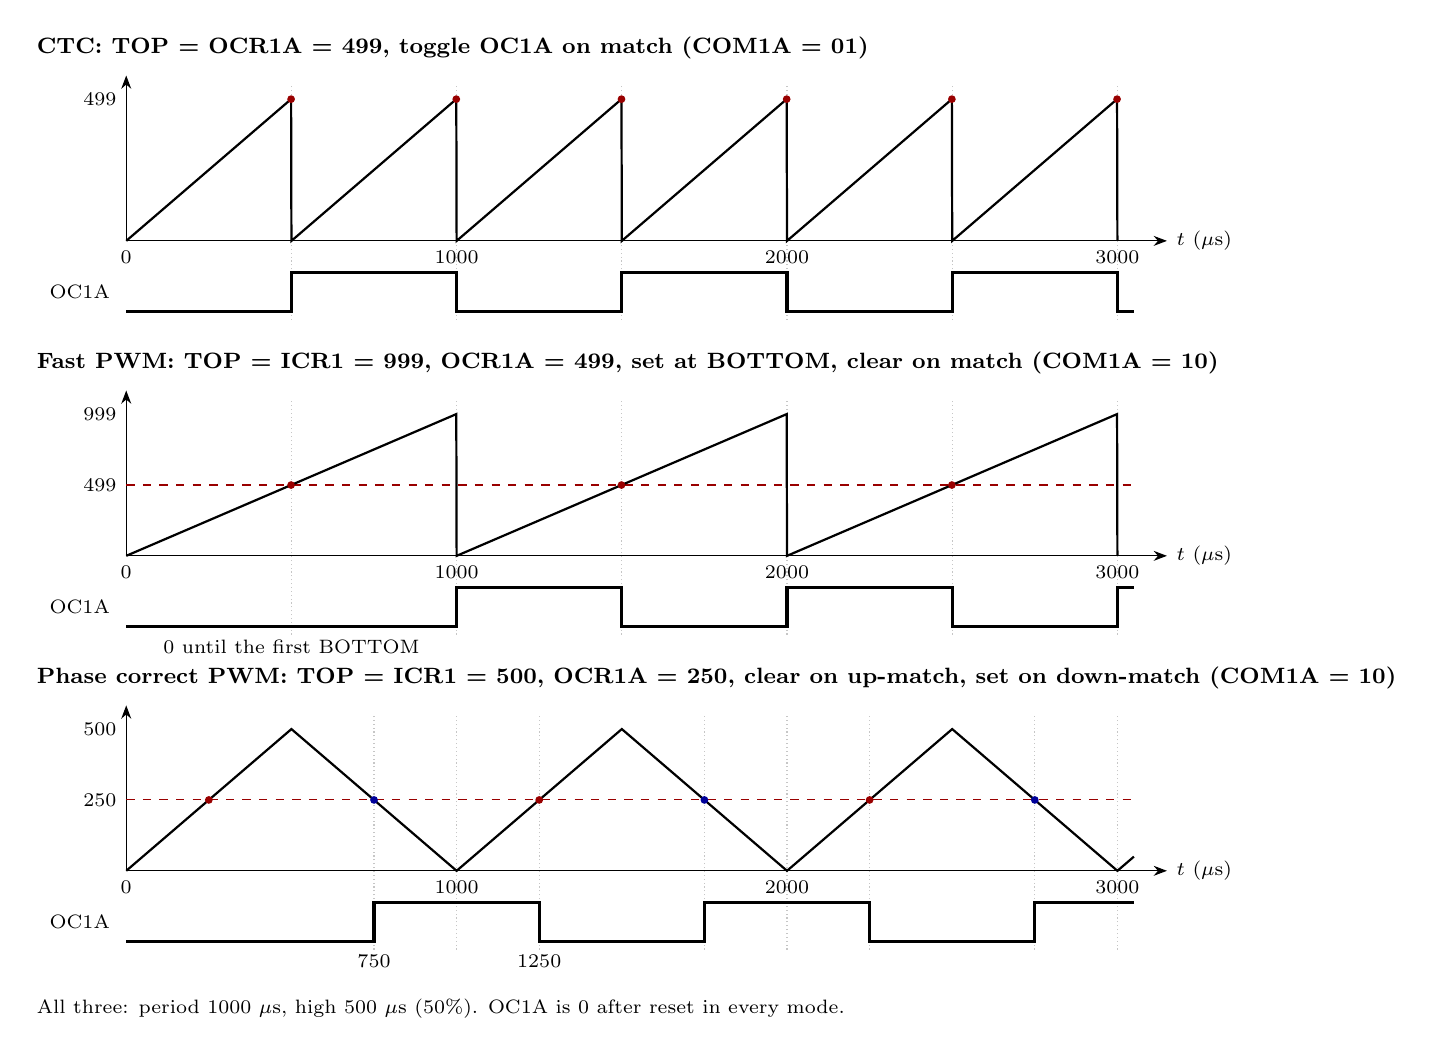
\begin{tikzpicture}[>=Stealth,font=\small,x=0.0042cm,y=1cm]
% 1 unit = 1 us (1 MHz, no prescaler). Each panel: TCNT1 (top) and OC1A (bottom), 0..3000 us.
\def\H{1.8}
% ---------- CTC ----------
\node[font=\footnotesize\bfseries,anchor=west] at (-300,2.45) {CTC: TOP = OCR1A = 499, toggle OC1A on match (COM1A = 01)};
\foreach \t in {500,1000,1500,2000,2500,3000} \draw[gray!45,densely dotted] (\t,-1.0) -- (\t,2.0);
\draw[->] (0,0) -- (0,2.1); \draw[->] (0,0) -- (3150,0) node[right,font=\scriptsize]{$t$ ($\mu$s)};
\node[anchor=east,font=\scriptsize] at (0,\H) {499};
\draw[thick] (0,0) \foreach \k in {1,...,6} { -- (\k*500-1,\H) -- (\k*500,0) };
\foreach \k in {1,...,6} \fill[red!60!black] (\k*500-1,\H) circle (1.4pt);
\foreach \t in {0,1000,2000,3000} \node[below,font=\scriptsize] at (\t,0) {\t};
\begin{scope}[yshift=-0.9cm]
\node[anchor=east,font=\scriptsize] at (-20,0.25) {OC1A};
\draw[very thick] (0,0) -- (500,0) -- (500,0.5) -- (1000,0.5) -- (1000,0) -- (1500,0) -- (1500,0.5) -- (2000,0.5) -- (2000,0) -- (2500,0) -- (2500,0.5) -- (3000,0.5) -- (3000,0) -- (3050,0);
\end{scope}
% ---------- Fast PWM ----------
\begin{scope}[yshift=-4.0cm]
\node[font=\footnotesize\bfseries,anchor=west] at (-300,2.45) {Fast PWM: TOP = ICR1 = 999, OCR1A = 499, set at BOTTOM, clear on match (COM1A = 10)};
\foreach \t in {500,1000,1500,2000,2500,3000} \draw[gray!45,densely dotted] (\t,-1.0) -- (\t,2.0);
\draw[->] (0,0) -- (0,2.1); \draw[->] (0,0) -- (3150,0) node[right,font=\scriptsize]{$t$ ($\mu$s)};
\node[anchor=east,font=\scriptsize] at (0,\H) {999};
\node[anchor=east,font=\scriptsize] at (0,\H*499/999) {499};
\draw[red!60!black,dashed] (0,\H*499/999) -- (3050,\H*499/999);
\draw[thick] (0,0) \foreach \k in {1,2,3} { -- (\k*1000-1,\H) -- (\k*1000,0) };
\foreach \k in {0,1,2} \fill[red!60!black] (\k*1000+499,\H*499/999) circle (1.4pt);
\foreach \t in {0,1000,2000,3000} \node[below,font=\scriptsize] at (\t,0) {\t};
\begin{scope}[yshift=-0.9cm]
\node[anchor=east,font=\scriptsize] at (-20,0.25) {OC1A};
\draw[very thick] (0,0) -- (1000,0) -- (1000,0.5) -- (1500,0.5) -- (1500,0) -- (2000,0) -- (2000,0.5) -- (2500,0.5) -- (2500,0) -- (3000,0) -- (3000,0.5) -- (3050,0.5);
\node[font=\scriptsize,anchor=north] at (500,-0.05) {0 until the first BOTTOM};
\end{scope}
\end{scope}
% ---------- Phase correct ----------
\begin{scope}[yshift=-8.0cm]
\node[font=\footnotesize\bfseries,anchor=west] at (-300,2.45) {Phase correct PWM: TOP = ICR1 = 500, OCR1A = 250, clear on up-match, set on down-match (COM1A = 10)};
\foreach \t in {750,1000,1250,1750,2000,2250,2750,3000} \draw[gray!45,densely dotted] (\t,-1.0) -- (\t,2.0);
\draw[->] (0,0) -- (0,2.1); \draw[->] (0,0) -- (3150,0) node[right,font=\scriptsize]{$t$ ($\mu$s)};
\node[anchor=east,font=\scriptsize] at (0,\H) {500};
\node[anchor=east,font=\scriptsize] at (0,\H/2) {250};
\draw[red!60!black,dashed] (0,\H/2) -- (3050,\H/2);
\draw[thick] (0,0) -- (500,\H) -- (1000,0) -- (1500,\H) -- (2000,0) -- (2500,\H) -- (3000,0) -- (3050,\H*50/500);
\foreach \t in {250,1250,2250} \fill[red!60!black] (\t,\H/2) circle (1.4pt);
\foreach \t in {750,1750,2750} \fill[blue!60!black] (\t,\H/2) circle (1.4pt);
\foreach \t in {0,1000,2000,3000} \node[below,font=\scriptsize] at (\t,0) {\t};
\begin{scope}[yshift=-0.9cm]
\node[anchor=east,font=\scriptsize] at (-20,0.25) {OC1A};
\draw[very thick] (0,0) -- (750,0) -- (750,0.5) -- (1250,0.5) -- (1250,0) -- (1750,0) -- (1750,0.5) -- (2250,0.5) -- (2250,0) -- (2750,0) -- (2750,0.5) -- (3050,0.5);
\foreach \t in {750,1250} \node[font=\scriptsize,anchor=north] at (\t,-0.05) {\t};
\end{scope}
\end{scope}
\node[font=\scriptsize,anchor=north west] at (-300,-9.5) {All three: period 1000 $\mu$s, high 500 $\mu$s (50\%). OC1A is 0 after reset in every mode.};
\end{tikzpicture}
\end{document}
